
%(BEGIN_QUESTION)
% Copyright 2012, Tony R. Kuphaldt, released under the Creative Commons Attribution License (v 1.0)
% This means you may do almost anything with this work of mine, so long as you give me proper credit

This solvent storage tank is filled from the truck unloading rack, and emptied by pump P-25 pumping solvent at a constant flow rate to the solvent wash process:

$$\includegraphics[width=15.5cm]{i0006rx01.eps}$$

Level transmitter LT-305 monitors the volume of solvent stored in this tank.  Over a period of several hours, an operator makes a log of solvent volumes and times:

% No blank lines allowed between lines of an \halign structure!
% I use comments (%) instead, so that TeX doesn't choke.

$$\vbox{\offinterlineskip
\halign{\strut
\vrule \quad\hfil # \ \hfil & 
\vrule \quad\hfil # \ \hfil \vrule \cr
\noalign{\hrule}
%
% First row
Solvent volume & Time \cr
(gallons) & (hour:minute) \cr
%
\noalign{\hrule}
%
% Another row
2951 gallons & 2:45 \cr
%
\noalign{\hrule}
%
% Another row
2897 gallons & 3:05 \cr
%
\noalign{\hrule}
%
% Another row
2843 gallons & 3:25 \cr
%
\noalign{\hrule}
%
% Another row
2789 gallons & 3:45 \cr
%
\noalign{\hrule}
%
% Another row
2735 gallons & 4:05 \cr
%
\noalign{\hrule}
%
% Another row
3140 gallons & 4:25 \cr
%
\noalign{\hrule}
%
% Another row
3086 gallons & 4:45 \cr
%
\noalign{\hrule}
%
% Another row
3032 gallons & 5:05 \cr
%
\noalign{\hrule}
} % End of \halign 
}$$ % End of \vbox

\vskip 10pt

Your task is to determine the flow rate of solvent to the solvent wash process, the approximate time when the tank was re-filled, and the approximate re-fill flow rate from the supply truck.  Sketch the graphical interpretation of this calculus problem, showing how a graph makes visual sense of the given information as well as the final result.

\underbar{file i01922}
%(END_QUESTION)





%(BEGIN_ANSWER)

A graph shows the volume over time to look something like this:

$$\includegraphics[width=15.5cm]{i01922x01.eps}$$

The flow rate out of the tank to solvent wash may be found by calculating the rise-over-run of the slope prior to filling:

$${dV \over dt} \approx {\Delta V \over \Delta t} = {{2897 \hbox { gal} - 2951 \hbox{ gal}} \over {\hbox{3:05} - \hbox{2:45}}} = {-54 \hbox{ gal} \over 20 \hbox{ min}} = -2.7 \hbox{ gallons per minute}$$

The tank is obviously filled at some time between 4:05 and 4:25.  The exact slope (derivative) of volume over time is unknown to us, since the only data points we have are at 4:05 and 4:25 exactly, and it would be sheer coincidence if these times just happened to be the exact start and finish times of the truck's unloading operation.  However, we can estimate the average (net) flow rate into the tank during these two times using the same numerical differentiation procedure:

$${dV \over dt} \approx {\Delta V \over \Delta t} = {{3140 \hbox { gal} - 2735 \hbox{ gal}} \over {\hbox{4:25} - \hbox{4:05}}} = {405 \hbox{ gal} \over 20 \hbox{ min}} = 20.25 \hbox{ gallons per minute}$$

We must remember that estimations of flow into or out of a vessel based on changes in liquid volume within that vessel only yield {\it net} flow.  During the time this tank was being filled, it was probably still feeding the solvent wash process at -2.7 gallons per minute.  Therefore, the net flow rate we just calculated of 20.25 gallons per minute is the combination of the truck's unloading rate and the out-flow rate to solvent wash.  Therefore, the truck's average unloading rate is actually 20.25 GPM + 2.7 GPM = 22.95 gallons per minute.

%(END_ANSWER)





%(BEGIN_NOTES)

\vskip 20pt \vbox{\hrule \hbox{\strut \vrule{} {\bf Virtual Troubleshooting} \vrule} \hrule}

This question is a good candidate for a ``Virtual Troubleshooting'' exercise.  Presenting the diagram to students, you first imagine in your own mind a particular fault in the system.  Then, you present one or more symptoms of that fault (something noticeable by an operator or other user of the system).  Students then propose various diagnostic tests to perform on this system to identify the nature and location of the fault, as though they were technicians trying to troubleshoot the problem.  Your job is to tell them what the result(s) would be for each of the proposed diagnostic tests, documenting those results where all the students can see.

During and after the exercise, it is good to ask students follow-up questions such as:

\begin{itemize}
\item{} What does the result of the last diagnostic test tell you about the fault?
\item{} Suppose the results of the last diagnostic test were different.  What then would that result tell you about the fault?
\item{} Is the last diagnostic test the best one we could do?
\item{} What would be the ideal order of tests, to diagnose the problem in as few steps as possible?
\end{itemize}

%INDEX% Mathematics, calculus: differentiation (calculating rates of flow based on volume and time data)
%INDEX% Process: oily water sump (realistic P&ID shown)

%(END_NOTES)

